\begin{questions}

  \question 分析下述各种情况下物体受到的力以及这些力的反作用
  力(图\ref{fig:03.17})。
  \begin{figure}[h]
      \vspace{-1.5em}
    \centering
    \subfigure[]{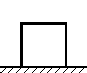
\includegraphics{figure/fig03.17a}\label{fig:03.17a}} \hspace{4em}
    \setcounter{subfigure}{2}
    \subfigure[]{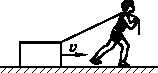
\includegraphics{figure/fig03.17c}}\\[1em]
    \setcounter{subfigure}{1}
    \subfigure[]{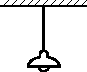
\includegraphics{figure/fig03.17b}} \hspace{4em}
    \setcounter{subfigure}{3}
    \subfigure[]{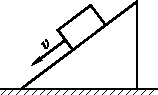
\includegraphics{figure/fig03.17d}}
    \caption{}
    \label{fig:03.17}
  \end{figure}

  (a) 静止在地面上的木箱;

  (b) 悬挂着的电灯;

  (c) 粗糙地面上被拖着走的重物;

  (d)沿固定的粗糙斜面下滑的物件。

  \question 物体所受的摩擦力的方向是否一定与它的运动方向相反?

  \question 木箱放在地面或斜面上,说明摩擦力的大小和方向。在下
  列几种情况中(图\ref{fig:03.18}),已知木箱质量为$ M $,与地面或斜面间的
  % 111.jpg
  静摩擦系数为 $ \mu _ { 0 } $  ,滑动摩擦系数为$ \mu $,斜面倾角为$ \alpha $ 。

  \begin{figure}[h]
    \vspace{-0.5em}
    \centering
    \subfigure[]{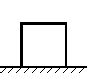
\includegraphics{figure/fig03.18a}} \hspace{4em}
    \setcounter{subfigure}{2}
    \subfigure[]{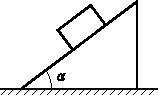
\includegraphics{figure/fig03.18c}}\\
    \setcounter{subfigure}{1}
    \subfigure[]{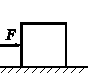
\includegraphics{figure/fig03.18b}} \hspace{4em}
    \setcounter{subfigure}{3}
    \subfigure[]{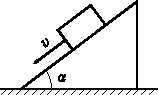
\includegraphics{figure/fig03.18d}}
    \caption{}
    \label{fig:03.18}
    \vspace{-0.5em}
  \end{figure}

  \begin{wrapfigure}[6]{r}{10em}
    \centering
    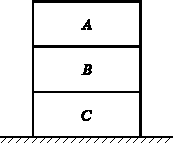
\includegraphics{figure/fig03.19}
    \caption{}
    \label{fig:03.19}
  \end{wrapfigure}
  (a) 静止在地面上

  (b) 用水平力$ F $推地面上的木箱,木箱不动;

  (c)静止在固定的斜面上;

  (d)固定的斜面上下滑。

  \question 如图\ref{fig:03.19}~所示,$ A $,$ B $,$ C $三块砖叠
  在一起,放在水平地面上不动,质量分别
  为$ m_A $, $ m _ B $,$ m_C $,分析
  这三块砖所受到的力。

  \begin{wrapfigure}[9]{r}{16em}
      \vspace{-2em}
    \centering
    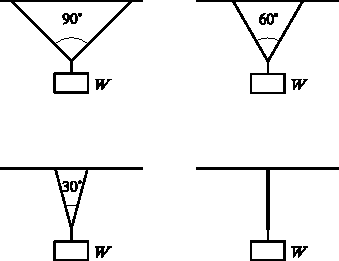
\includegraphics{figure/fig03.20}
    \caption{}
    \label{fig:03.20}
  \end{wrapfigure}
  \question 两个力的合力是否一定比其中任一个大?

  \question 同一重物用两根等长的绳悬挂起来,
  采取不同的角度,分别如图\ref{fig:03.20}~所示,哪一
  种情况绳所受的拉力最大?哪种最小?

  % 112.jpg
  \clearpage
  \question 自由下落的物体,在下列几种情况下,加速度如何?

  (1) 不考虑空气的阻力;

  (2) 考虑空气的阻力,但认为阻力的大小为恒量

  (3) 考虑空气的阻力,认为阻力的大小与速度大小成正比。

  \question 马拉车,车也拉马。根据牛顿第三定律,作用力与反作用
  力大小相等、方向相反,那么,为什么车及马整个体系能向前走?

  \question 电梯中有质量为$ m $的物体,求下述各种情况中物体对电梯
  底部的压力:

  (1) 电梯静止;

  (2) 电梯匀速上升;

  (3) 电梯以加速度$ a $上升;

  (4) 电梯以加速度$ a $下降。

  \question 现在我们知道,物质表面的磨光程度有一个限度,如果超
  过这一限度,反而增加摩擦阻力。试解释这一事实。

  \question 在光滑的冰上走路,用小步还是用大步走好?为什么?

  \question 一个人静止在结冰的湖面上,如果冰面是完全光滑的(即
  人与冰面之间没有摩擦力)。试问他怎样才能到达岸上?

  \question 一轻绳跨过一个定滑轮,绳的两端各被一个猴子抓住。这
  两个猴子重量相等。开始时处在同一高度,试考虑:

  (1) 猴子甲能否往上爬而将猴子乙丢在比自己低的高度上?

  \begin{wrapfigure}[5]{r}{10em}
    \centering
    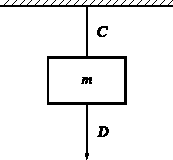
\includegraphics{figure/fig03.21}
    \caption{}
    \label{fig:03.21}
  \end{wrapfigure}
  (2) 猴子甲能否沿着绳往下滑而将猴子乙留在比自己高的高
  度上?

  (3) 猴子甲放开绳子,能否比猴子乙早落到地上?

  \question 如果取力、长度、时间为基本量,
  则质量的量纲是什么?

  \question 物体运动时所受的阻力可写成
  \begin{equation*}
      F = \beta v ^ n
  \end{equation*}
  % 113.jpg
  其中$ F $是阻力;$ v $是速度;$ n $为某个数。在低速时$  n = 1  $, $ \beta $  是一个
  常数。试求$ \beta $的量纲。

  \question 如图\ref{fig:03.21}~所示,用一弦线将质量为$ m $的物体挂在天花板
  上,再用同样质地的弦线$ D $系在$ m $下面。试说明以下事实

  (1) 如果突然向下扯$ D $,$ D $就断;

  (2)如果慢慢地向下扯$ D $,则$ C $先断。
\end{questions}



